\chapter{Rule Set Language}
\label{chaprulelang}

The rule set language forms the core of \GrG. Rule files refer to zero\footnote{Omitting a graph model means that \GrG\ uses a default graph meta model. The default model consists of the base type \texttt{Node} for vertices and the base type \texttt{Edge} for edges.} or more graph models and specify a set of rewrite rules. The rule language covers the pattern specification and the replace/modify specification. Attributes of graph elements can be re-evaluated during a rule application. The following rewrite rule from \cite{geiss} gives a rough picture of the language:
%\begin{figure}[tb]
\begin{example}\label{ex:rule:SomeRule}
\begin{grgen}
actions SomeActions using SomeModel;

rule SomeRule {
  pattern {
    n1 : NodeTypeA;
    n2 : NodeTypeA;
    hom(n1, n2);
    n1 --> n2;
    n3: NodeTypeB;
    negative {
      n3 -e1:EdgeTypeA-> n1;
      if {n3.a1 == 42*n2.a1;}
    }
    negative {
      n4: Node \ (NodeTypeB);
      n3 -e1:EdgeTypeB->n4;
      if {typeof(e1) >= EdgeTypeA;}
    }
  }
  replace {
    n5: NodeTypeC<n1>;
    n3 -e1:EdgeTypeB-> n5;
    eval {
      n5.a3 = n3.a1*n1.a2;
    }
  }  
}
\end{grgen}
\end{example}
%\end{figure}
In this chapter we use excerpts of example~\ref{ex:rule:SomeRule} (\texttt{SomeRule}) in further descriptions.

\section{Building Blocks}
\label{rulebb}

The \GrG\ rule set language is case sensitive. The language makes use of several identifier specializations in order to denominate all the \GrG\ entities.\\
\\
\emph{Ident}, \emph{IdentDecl}\\ \nopagebreak
A non-empty character sequence of arbitrary length consisting of letters, digits or underscores. The first character must not be a digit. \emph{Ident} may be an identifier defined in a graph model (see \ref{modelbb}). \emph{Ident} and \emph{IdentDecl} differ in their role: While \emph{IdentDecl} is a \emph{defining} occurrence of an identifier, \emph{Ident} is a \emph{using} occurrence. An \emph{IdentDecl} non-terminal can be annotated. See \ref{annotations} for annotations of declarations.
\begin{note}
  The \GrG\ rule set language does not distinguish between declarations and definitions. More precisely, every declaration is also a definition. That means, that every element of a LHS (left hand side, see section \ref{patternpart}) is actually mapped by a match. 
\end{note}
\mbox{ }\\
\emph{ModelIdent}, \emph{TypeIdent}, \emph{NodeType}, \emph{EdgeType}\\
These are (semantic) specializations of Ident. \emph{TypeIdent} matches every type identifier, i.e. a node type, an edge type, an enum type or a primitive type. All the type identifiers are actually type \emph{expressions}. See \ref{typeexpressions} for the use of type expressions.\\

\begin{rail}
  Graphlet: GraphletNode (() | Continuation) ';' ;
  Continuation: GraphletEdge GraphletNode (() | Continuation) ;
\end{rail}
A graphlet specifies a connected subgraph. With graphlets \GrG\ provides a descriptive notation to define both, patterns to search for as well as the subgraphs that replace/modify a pattern. A pattern graphlet is specified piecewise. In our example the statement \texttt{n1 --> n2} is the node identifier \texttt{n1} followed by the pattern continuation \texttt{--> n2}. In addition to the graphlet specification itself, you can bind names to your defined graph elements. So \GrG\ selects graph elements either
\begin{itemize}
  \item by its type:\\
     for instance \texttt{v:NodeType1 -e:EdgeType-> w:NodeType2} selects some node of type \texttt{Node\-Type1} that is connected to a node of type \texttt{NodeType1} by an edge of type \texttt{EdgeType} and binds the names \texttt{v}, \texttt{w}, and \texttt{e}
   \item[ ] or
   \item by its name. \\
     That is  \texttt{v -e-> w} selects the specific graph elements the names \texttt{v}, \texttt{w}, and \texttt{e} are bound to. Of course those names have to be defined. 
\end{itemize}
Binding of names is optional. In case of omitting a name the graph element is called \emph{anonymous}. Anonymous graph elements get an internal, non-accessible name. For illustration purposes we use a \texttt{\$<number>} notation to denote anonymous graph elements in this document.\\
Binding of names also allows for splitting a single graphlet into multiple graphlets.
\begin{example}
The following graphlet (\texttt{n1}, \texttt{n2}, and \texttt{n3} are defined somewhere)
\begin{grgen}
n1 --> n2 --> n3 <-- n1;
\end{grgen}
is equivalent to
\begin{grgen}
n1 --> n3;
n1 --> n2;
n3 <-- n1;
\end{grgen}
\end{example}

\begin{rail}
GraphletNode: (() |
    Ident | 
    (() | IdentDecl) ':' NodeType (() | TypeConstraint | '<' Ident '>')) ;   
\end{rail}
Specifies a node of type \emph{NodeType} with respect to \emph{TypeConstraint} (see section \ref{typeexpressions}, \emph{TypeConstraint}). Type constraints are allowed in the pattern part only. If \emph{NodeType} is omitted, the base type \texttt{Node} is assumed. Remember that every node type has \texttt{Node} as super type. The \texttt{<>} operator retypes a node. Retyping is allowed in the replace/modify part only (see section \ref{replacepart}, \emph{Retyping}).
\begin{center}
  \begin{tabular}[c]{ll}
    \textbf{Graphlet} & \textbf{Meaning}\\ \hline
    \texttt{x:NodeType;} & The name \texttt{x} is bound to a node of type \texttt{NodeType} or one of its subtypes. \\
    \texttt{ :NodeType;} & \texttt{\$1:NodeType} \\
    \texttt{ ;} & \texttt{\$1:Node} \\
    \texttt{x;} & The node \texttt{x} is bound to.
  \end{tabular}
\end{center} 

\begin{rail}
  GraphletEdge: '-' EdgeRefinement '->'  | '<-' EdgeRefinement '-' ;
  EdgeRefinement: () | Ident | (() | IdentDecl) ':' EdgeType (() | TypeConstraint | '<' Ident '>') ;
\end{rail}
Specifies an edge. Anonymous edges are specified by \texttt{-->} or \texttt{<--}. For a more detailed specification you can use an edge refinement clause between the arrow dashes. Type constraints are allowed in the pattern part only (see section \ref{typeexpressions}, \emph{TypeConstraint}). The \texttt{<>} operator retypes an edge. Retyping is allowed in the replace/modify part only (see section \ref{replacepart}, \emph{Retyping}).\\
Edges are never specified separately. Instead selecting an edge always means selecting its incident nodes, too.
\begin{center}
  \begin{tabular}[c]{ll}
    \textbf{Graphlet} & \textbf{Meaning}\\ \hline
    \texttt{-e:EdgeType-> ;} & \texttt{\$1:Node -e:EdgeType-> \$2:Node;} (Schleifen?)  \\
    \texttt{ -:EdgeType-> ;} & \texttt{\$1:Node -\$2:EdgeType-> \$3:Node;} \\
    \texttt{ --> ;} & \texttt{\$1:Node -\$2:Edge-> \$3:Node;} \\
    \texttt{ -e-> ;} & The edge \texttt{e} is bound to and its incident nodes.
  \end{tabular}
\end{center} 

\begin{figure}[htbp]
\begin{example}
Some graphlets:

\centering
\begin{tabular}[c]{cl}
  & \\
  \begin{tabular}[c]{c}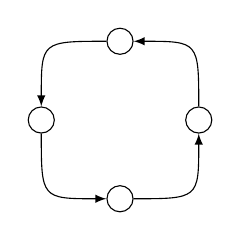
\begin{tikzpicture}
      \tikzstyle{every node}=[circle]
      \node[draw] (n1) at (1,0) {};
      \node[draw] (n2) at (2,1) {};
      \node[draw] (n3) at (1,2) {};
      \node[draw] (n4) at (0,1) {};
    	
      \draw[-latex] (n3) .. controls +(-1,0) .. (n4) {};
      \draw[-latex] (n4) .. controls +(0,-1) .. (n1) {};
      \draw[-latex] (n1) .. controls +(1,0) .. (n2) {};
      \draw[-latex] (n2) .. controls +(0,1) .. (n3) {};
    \end{tikzpicture}\end{tabular} & \begin{tabular}[c]{l} \texttt{x:Node --> --> --> --> x;} \end{tabular}\\
  & \\  
  \begin{tabular}[c]{c}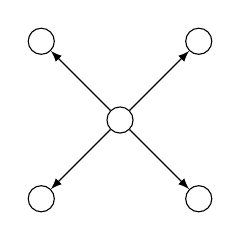
\begin{tikzpicture}
      \tikzstyle{every node}=[circle]
      \node[draw] (n1) at (1,1) {};
      \node[draw] (n2) at (0,0) {};
      \node[draw] (n3) at (0,2) {};
      \node[draw] (n4) at (2,0) {};
      \node[draw] (n5) at (2,2) {};
    	
      \draw[-latex] (n1) -- (n2) {};
      \draw[-latex] (n1) -- (n3) {};
      \draw[-latex] (n1) -- (n4) {};
      \draw[-latex] (n1) -- (n5) {};
    \end{tikzpicture}\end{tabular} & \begin{tabular}[c]{l} \texttt{<-- x:Node -->;} \\ \texttt{<-- x -->;} \end{tabular}\\
  & \\
  \begin{tabular}[c]{c}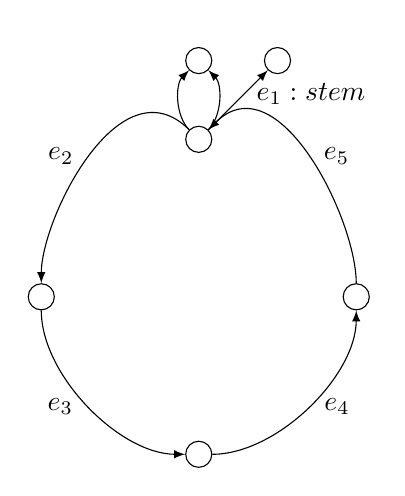
\begin{tikzpicture}
      \tikzstyle{every node}=[circle]
      \node[draw] (n1) at (3,5) {};
      \node[draw] (n2) at (2,4)   {};
      \node[draw] (n3) at (0,2)   {};
      \node[draw] (n4) at (2,0)   {};
      \node[draw] (n5) at (4,2)   {};
      \node[draw] (n6) at (2,5.0)   {};
    	
    	\draw[-latex] (n2) --                                  (n1) node[right,pos=0.6] {$e_1:\text{stem}$};
    	\draw[-latex] (n2) .. controls +(-1,1) and +(0,1) ..   (n3) node[left,midway]  {$e_2$};
      \draw[-latex] (n3) .. controls +(0,-1) and +(-1,0) ..  (n4) node[left,midway]  {$e_3$};
    	\draw[-latex] (n4) .. controls +(1,0)  and +(0,-1) ..  (n5) node[right,midway] {$e_4$};
      \draw[-latex] (n5) .. controls +(0,1)  and +(1,1) ..   (n2) node[right,midway] {$e_5$};
    	\draw[-latex] (n2) .. controls +(-0.3,+0.3) and +(-0.3,-0.3) .. (n6) node[left,midway]   {};
    	\draw[-latex] (n2) .. controls +(+0.3,+0.3) and +(+0.3,-0.3) .. (n6) node[right,midway]  {};
    \end{tikzpicture}\end{tabular} & \begin{tabular}[c]{l} \texttt{<-e1:stem- n1:Node -e2:Edge-> -e3:Edge->} \\ \quad\texttt{-e4:Edge-> -e5:Edge-> n1;}\\ \texttt{n1 --> n2:Node;} \\ \texttt{n1 --> n2;} \end{tabular}\\
   & \\
  \begin{tabular}[c]{c}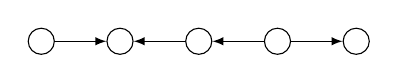
\begin{tikzpicture}
      \tikzstyle{every node}=[circle]
      \node[draw] (n1) at (0,0) {};
      \node[draw] (n2) at (1,0) {};
      \node[draw] (n3) at (2,0) {};
      \node[draw] (n4) at (3,0) {};
      \node[draw] (n5) at (4,0) {};
    	
      \draw[-latex] (n1) -- (n2) {};
      \draw[-latex] (n3) -- (n2) {};
      \draw[-latex] (n4) -- (n3) {};
      \draw[-latex] (n4) -- (n5) {};
    \end{tikzpicture}\end{tabular} & \begin{tabular}[c]{l} \texttt{--> <-- <-- --> ;} \end{tabular}
\end{tabular}
\end{example}
\end{figure}

\begin{note}
Although both, the pattern part and the replace/modify part, use graphlets, there are subtle changes between them. It concerns the \emph{TypeConstraint} clause, the retype operator \texttt{<>}, and the scope of defined graph element names: Names defined within the pattern part are valid in the pattern part as well as in the replace/modify part. Names defined within the replace/modify part are unknown to the pattern part.
\end{note}

\section{Rules and Tests}
\label{ruledecls}
\begin{rail}
  'actions' IdentDecl (() | 'using' ((ModelIdent)+',')) ';' \\ ((TestDeclaration | RuleDeclaration)+) ;
\end{rail}
A rule set consists of the underlying graph models and several rewrite rules. In case of multiple graph models \GrG\ uses the union of these models. In this case beware of conflicting declarations. There is no built-in conflict resolution mechanism like packages or namespaces for models. If necessary you could use prefixes as you might do it in C.

\begin{rail}
  TestDeclaration: 'test' ActionSignature lbrace Pattern rbrace ;
  RuleDeclaration: 'rule' ActionSignature lbrace Pattern Replace rbrace ;
\end{rail}
Declares a single rewrite rule such as \texttt{SomeRule}. It consists of a pattern part (see \ref{patternpart}) in conjunction with its rewrite/modify part (see \ref{replacepart}). A test rule has no rewrite specification. It's intended to test whether (and maybe how many times) a pattern occurs.
\begin{example}
We define a test rule \texttt{SomeCond}
\begin{grgen}
test SomeCond {
  pattern {
    n: SeldomNodeType;
  }
}
\end{grgen}
and execute in \GrShell:
\begin{grshell}
  grs SomeCond & SomeRule
\end{grshell}
SomeRule will only be executed, if a node of type \texttt{SeldomNodeType} exists. For regular graph rewriting sequences in \GrShell\ see \ref{grsthings}.
\end{example}

\begin{rail}  
  ActionSignature: IdentDecl (() | Parameters) (() | ':' ReturnTypes) ;
\end{rail}
The signature sets the name of a rewrite rule to \emph{IdentDecl}. Additionally you can provide parameters to the rule and specify return types.

\begin{rail}
  Parameters: '(' (IdentDecl ':' (NodeType | EdgeType) + ',') ')' ;
  ReturnTypes: '(' ((NodeType | EdgeType) + ',') ')' ;
\end{rail}
Parameters are treated as (predefined) graph elements of the pattern. Even if a supplied parameter value is undefined, it is treated as valid node or edge definition. So in any case a graph element of the specified type has to be matched.
\begin{example}
Assume the following rule:
\begin{grgen}
rule r(e: Edge; x: Node) {
  pattern {
    x --> ;
  }
  modify {}
}
\end{grgen}
If \texttt{x} and \texttt{e} are undefined, rule \texttt{r} is equivalent to rule \texttt{s}:
\begin{grgen}
rule s {
  pattern {
    x:Node --> ;
    -e:Edge-> ;
  }
  modify {}
}
\end{grgen}
In particular \texttt{x} will not be incident to \texttt{e}.
\end{example}
The return types specify edge and node types of graph elements that are returned by the replace/modify part. If return types are specified, the \texttt{return} statement is mandatory. Otherwise no \texttt{return} statement must occur. If no pattern is found, the return values are undefined. See also section \ref{replacepart}, \texttt{return}.
\begin{example}
We extend \texttt{SomeRule} with a variable node to find and we want it to return the rewritten graph elements \texttt{n5} and \texttt{e1}.
\begin{grgen}
  rule SomeRuleExt(varnode: Node): (Node, EdgeTypeB) {
    pattern {
      n1: NodeTypeA;
      ...
    }
    replace {
      varnode;
      ...  
      return(n5, e1);
      eval {
        ...
\end{grgen}
We don't define \texttt{varnode} within the pattern part because this is already covered by the parameter specification itself.
\end{example}

\section{Pattern Part}
\label{patternpart}
\begin{rail}
  Pattern: 'pattern' lbrace (()+PatternStatement) rbrace ;
\end{rail}
A pattern consists of zero or more pattern statements. All the pattern statements must be fulfilled by a subgraph of the host graph in order to form a match. Even stronger -- a graph element of the host graph, that is matched by a statement, is ``bound'', i.e.\ it cannot be part of another pattern statement, unless you use the \texttt{hom} operator. An empty pattern always produces exactly one (empty) match.\\
Pattern statements may define names for graph elements for use by other pattern statements or replace statements. Such names may be used before their declaration.
\begin{note}
The application of a rule is not deterministic (remember the example in \ref{ov:example}), specifically there may be more than one subgraph that matches the pattern and any of them may be selected. The \LibGr\ provides several mechanisms in order to deal with such ambiguities (and so does the \GrShell). See section \ref{grsthings} for further information.
\end{note}

\begin{rail}  
  PatternStatement: 
    Graphlet ';' |
    'hom' '(' (Ident + ',') ')' ';' |
    'negative' lbrace (()+PatternStatement) rbrace |
    'if' lbrace (BooleanExpr ';' +) rbrace |
    'return' '(' (Ident+',') ')' ';' ;
\end{rail}
The semantics of the various pattern statements:
\begin{description}
  \item[Graphlet.] Graphlets specify connected subgraphs. See section \ref{rulebb} for a detailed explanation of graphlets. 
  \item[Isomorphic/Homomorphic Matching.] The \texttt{hom} operator specifies the nodes or edges that may be matched homomorphically. In contrast to the default isomorphic matching, the specified graph elements \emph{may} be mapped to the same graph element in the host graph. Note that the graph elements shall have a common supertype. Several homomorphically matched graph elements will be mapped to a graph element of a common subtype.\\
  In our example \texttt{n1} and \texttt{n2} may be the same node. This is possible because they are of the same type (\texttt{NodeTypeA}).
  \item[Negative Application Conditions (NACs).] With negative application conditions (keyword \texttt{negative}) we can specify graph patterns which forbid the application of a rule if any of them is present in the host graph (cf. \cite{adam}). NACs may not be nested. NACs possess an own scope. That means, names defined within a NAC are not alive outside the NAC. Identifiers from surrounding scopes may be overwritten.\\
  In our example the second negative condition uses \texttt{n3} from the surrounding scope and defines \texttt{n4} and \texttt{e1}. We may safely reuse the variable name \texttt{e1} in the replace part.
  \item[Attribute Conditions.] The Java-like attribute conditions (keyword \texttt{if}) in the pattern part allow for further restriction of the applicability of a rule.
  \item[Return values.] The return statement is only allowed for \texttt{test} rules. Otherwise the \texttt{return} statement belongs to the replace part. See \ref{replacepart}, \emph{Return Values}.
\end{description}
Keep in mind that using type constraints or the \texttt{typeof} operator might be helpful. See section \ref{typeexpressions} for further information.

\section{Replace/Modify Part}
\label{replacepart}
For the task of rewriting \GrG\ provides two different modes: A replace mode and a modify mode.
\begin{description}
  \item[Replace mode.] The semantics of this mode is to delete every graph element of the pattern that is not used (denoted) in the replace part, keep every graph element that is used, and create every additionally defined graph elements.\\
  In our example \texttt{SomeRuleExt} the nodes \texttt{varnode} and \texttt{n3} will be kept. The node \texttt{n1} is replaced by the node \texttt{n5} preserving \texttt{n1}'s edges. The anonymous edge instance between \texttt{n1} and \texttt{n2} only occurs in the pattern and therefore gets deleted.
  \item[Modify mode.] The modify mode can be regarded as a replace part in replace mode, where every pattern graph element is added (denoted) before the first replace statement. Additionally this mode supports the \texttt{delete} operator that deletes every element given as an argument. Deletion takes place after all other rewrite operations. Multiple deletion of the same graph element is allowed (but pointless) as well as deletion of just created elements (pointless, too).
\begin{example}
How might our example look in modify mode? We have to denominate the anonymous edge between \texttt{n1} and \texttt{n2} in order to delete it. The node \texttt{varnode} should be omitted. So we have
\begin{grgen}
rule SomeRuleExtMod(varnode: Node): (Node, EdgeTypeB) {
  pattern {
    ...
    n1 -e0:Edge-> n2;
    ...
  }
  modify {
    n5 : NodeTypeC<n1>;
    n3 -e1:EdgeTypeB-> n5;
    delete(e0);
    eval {
      ...
\end{grgen}
\end{example}
\end{description}

\begin{rail}
  Replace: ('replace' | 'modify') lbrace (()+ReplaceStatement) rbrace ;
\end{rail}
Selects whether the replace mode or the modify mode is used. Several replace statements describe the transformation from the pattern subgraph to the destination subgraph.

\begin{rail}  
  ReplaceStatement: Graphlet ';' |
    'delete' '(' (Ident + ',') ')' ';' |
    'eval' lbrace (Assignment ';' +) rbrace |
    'return' '(' (Ident+',') ')' ';' ;
\end{rail}    
The semantics of the various pattern statements:
\begin{description}
  \item[Graphlet.] Analogous to a pattern graphlet, a specification of a connected subgraph. Its graph elements are either kept because they are elements of the pattern or added otherwise. Names defined in the pattern part must not be redefined in the replace graphlet. See section \ref{rulebb} for a detailed explanation of graphlets. 
  \item[Deletion.] The \texttt{delete} operator is only available in the modify mode. It deletes the specified pattern graph elements. Multiple occurrences of \texttt{delete} statements are allowed. Deletion statements are executed after all other replace statements. Multiple deletion of the same graph element is allowed (but pointless) as well as deletion of just created elements (pointless, too).
  \item[Attribute Evaluation.] If a rule is applied, then the attributes of matched and inserted graph elements will be recalculated.
  \item[Return Values.] Graph elements of the replace part can be returned according to the return types in the signature (see \ref{ruledecls}, \texttt{ActionSignature}). The \texttt{return} statement must not occur multiple times. The graph element names have to be in the same order as the corresponding return types in the signature. The named elements must be compatible to the declared type.
  \item[Retyping.] Retyping enables us to keep all adjacent nodes and all attributes stemming from common super types of a graph element while changing its type. Retyping differs from a type cast: During replacement both of the graph elements are alive. Specifically both of them are available for evaluation. Furthermore the source and destination types need not to be on a path in the directed type hierarchy tree, rather their relation can be arbitrary.\\
The edge specification as well as \emph{ReplaceNode} supports retyping. In our example node \texttt{n5} is a retyped node stemming from node \texttt{n1}.
\end{description} 

\begin{rail}    
   Assignment: Ident '.' Ident '=' Expression ;
\end{rail}
Several evaluation parts are allowed within the replace part. Multiple evaluation statements will be internally concatenated, preserving their order. Evaluation statements have imperative semantics. Especially \GrG\ does not care about data dependencies. Evaluation takes place before any graph elements get deleted and after every new element has been created. You may read (and write, although this doesn't make sense) attributes of graph elements to be deleted.
\begin{example}
\begin{grgen}
...
replace{
  ...
  eval {y.i = 40;}
  eval {y.j = 0;}
  x: IJNode;
  y: IJNode;
  delete(x);
  eval {
    x.i = 1; 
    y.j = x.i;
    x.i = x.i + 1;
    y.i = y.i + x.i;
  }
\end{grgen}
This nonsense example yields to $y.i = 42$, $y.j = 1$.
\end{example}

